\begin{mybilan}
	
	\twoCol{
	\begin{center}
		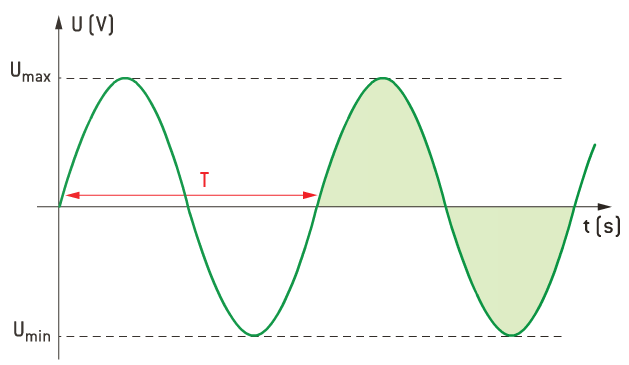
\includegraphics[scale=0.6]{bilan4}
	\end{center}

	\begin{itemize}
		\item Une \kw{tension alternative} prend des \kw{valeurs positives puis négatives qui se compensent} au cours du temps.
		\item Le graphique d'une tension sinusoïdale a une forme caractéristique, observée sur le schéma.
		\item La \kw{tension maximale $\mathbf{U_{max}}$} est la plus grande valeur de la tension.
		\item La \kw{tension maximale $\mathbf{U_{min}}$} est la plus petite valeur de la tension.
	\end{itemize}
	}

\end{mybilan}